\documentclass{report}

\usepackage{amsmath}
\usepackage[german]{babel}
\usepackage{amssymb}
\usepackage{amsxtra}
\usepackage[dvips]{epsfig,psfrag}
\usepackage{listings}
\usepackage{pdfpages}

\newcommand{\refchapter}[1]{Kapitel~\ref{#1}}
\newcommand{\refsec}[1]{Sektion~\ref{#1}}
\newcommand{\refeqn}[1]{Gleichung~(\ref{#1})}
\newcommand{\reffig}[1]{Abbildung~\ref{#1}}
\renewcommand{\arraystretch}{1.5}

\title{\bf CES Softwareentwicklungspraktikum \\
{\small Analyse- und Entwurfsdokument} \vspace{1cm}\\

\epsfig{file=figures/cces_logo.eps,width=\textwidth}
}


\author{Lena Blum, Alexander Fischer und William Hulin}
\date{Matr.-Nr. 302253, 303979 und 293858 \\
email: {\tt [lena.blum|alexander.fischer|william.hulin]@rwth-aachen.de} 
}

\begin{document}
\parindent 0pt
\lstloadlanguages{[ISO]C++}
\lstset{basicstyle=\small, numbers=left, numberstyle=\footnotesize,
  stepnumber=1, numbersep=5pt, breaklines=true, escapeinside={/*@}{@*/}}


\pagestyle{headings}

\maketitle

\tableofcontents


\chapter{Vorwort}
\label{ch:1}

\section{Aufgabenstellung und Struktur des Dokuments}
\label{sec:1.1}

\subsection*{Aufgabenstellung}

{Im Rahmen des Softwareentwicklungspraktikums (CES$\_$SS2012) soll eine Software zur Simulation eines Stehaufkreisels erstellt werden.
Die Simulationssoftware muss sowohl den reibungsfreien, als auch den reibungsbehafteten Fall korrekt simulieren können.

Als Programmiersprache soll C++ verwendet werden. Der Quellcode soll derart strukturiert
und kommentiert sein, dass sp\"atere Modifikationen und Erweiterungen durch Dritte m\"oglich sind.}

\section{Projektmanagement}
\label{sec:1.2}

{
\begin{tabular}{l || l}
  \hline
  \hline
	Protoyping (MATLAB/ FORTRAN)& Alexander \\
	\hline
	Dokumentation &Lena \\
	\hline
	\hline
	Coding:& \\
	\hline
	Parameterset, Solver, Solution, Rkv56Parset, Rkv56,\\ DESolution,\textless  \textless interface\textgreater \textgreater RightSide, RHS, Rkv56Modified & Alexander\\
	\hline
	\textless \textless interface \textgreater \textgreater OutputInterface, OutputToolbox, Main, ExceptionHandlingModule,\\ MathException, NonCriticalME, CriticalME, ParameterException & William\\
	\hline
	GUI & Lena \\
	\hline
	\hline
\end{tabular}
}

\section{Lob und Kritik}
\label{sec:1.3}

{\em - folgt -}


\chapter{Analyse}
\label{ch:2}

\section{Anforderungsanalyse}
\label{sec:2.1}

\subsection{Benutzeranforderungen}

{Das von Herrn Professor Gauger gestellte Simulationsproblem umfasst die Erstellung einer Software zur Simulation eines Stehaufkreisels.

Die Simulation muss sowohl den reibungsbehafteten, als auch reibungsfreien Fall korrekt simulieren.

Im Speziellen wird ein Runge-Kutta56-Verfahren mit adaptiver Schrittweitensteuerung unter Betrachtung einer Erhaltungsgr\"o\ss e (\textit{conserved quantity}) zur Simulation des Problems verwendet.\\ 
\textit{Wahrscheinlich wird das Rkv56 Verfahren durch ein BDF-Verfahren oder eine C++ Implementierung eines speziellen Krylow-Verfahrens ersetzt.\\
https://computation.llnl.gov/casc/software.html } \\ 
Die Realisierung der Simulation findet in C++ statt. \\

Die Bedienung sowie das ausgeben der Simulationsergebnisse muss durch eine grafische Benutzeroberfl\"ache (\textit{GUI}) m\"oglich sein.

Die Simulationsergebnisse k\"onnen in einer \textit{ASCII}-formatierten Datei zur weiteren Verarbeitung und Auswertung exportiert werden.

Durch den modularen Aufbau ist die Wartbarkeit und einfache Erweiterbarkeit der Software durch Dritte gew\"ahrleistet.
 

Das Kernproblem besteht im L\"osen der Rechten Seite des folgenden Differentialgleichungssystems:

\begin{align*}
	&
	\ddot \theta (I+ma^2\sin^2\theta+kma\sin \theta(R-a\cos\theta)(-\dot x_c
	\sin\phi+\dot y_c \cos \phi-(R-a\cos\theta)\dot \theta))
	\\&
	=\underbrace{-(I_3-I)\dot \phi^2\sin\theta\cos\theta}_{=0}-I_3\dot \phi \sin \theta \dot \psi 
	+ (g+a\dot \theta^2\cos \theta)(-ma\sin\theta - km(R-a\cos \theta)
	\\&
	(-\dot x_c \sin \phi +\dot y_c \cos \phi-(R-a\cos\theta)\dot \theta))
\end{align*}
\begin{align*}
	&
	\ddot \phi I \sin\theta= -\underbrace{(2I-I_3)}_{=I}
	\dot \phi \dot \theta \cos \theta + I_3\dot \theta \dot \psi
	\\&
	-km(g+a\cos\theta\dot\theta^2+a\sin\theta\ddot\theta)
	(a-R\cos\theta)(\dot x_c\cos \phi +\dot y_c \sin\phi+
	(a\dot \phi+\dot \psi R)\sin \theta)
\end{align*}
\begin{align*}
	&\ddot \psi I_3=-I_3(\ddot \phi \cos \theta - \dot \phi \dot \theta \sin \theta)
	\\&
	-km(g+a\cos\theta\dot\theta^2+a \sin\theta\ddot \theta)(R\sin\theta)
	(\dot x_c\cos \phi +\dot y_c \sin \phi+(a\dot \phi +\dot \psi R)\sin\theta)
\end{align*}
\begin{align*}
	&m\ddot x_c=-km(g+a\cos\theta\dot \theta^2+a\sin \theta\ddot\theta)
	(\dot x_c+(a\dot \phi + \dot \psi R)\sin \theta\cos \phi+
	(a\cos \theta -R)\sin \phi \dot \theta)
\end{align*}
\begin{align*}
	&m\ddot y_c=-km(g+a\cos \theta\dot \theta^2+a \sin \theta \ddot \theta)
	(\dot y_c+(a\dot \phi + \dot \psi R)\sin \theta \cos \phi
	+(R-a\cos \theta)\cos\phi \dot \theta)
\end{align*} }

\subsection{Systemanforderungen}
%% \subsection{Anwendungsfallanalyse}


\subsubsection{Funktionale Anforderungen}

{Dem Anwender ist es m\"oglich die Simulationsparameter k (Reibung) sowie 
$ \dot \psi $ (rad/s) \"uber eine grafische Eingabemaske festzulegen. 
Wenn w\"ahrend der Simulation ein Fehler auftritt wird der Anwender 
\"uber ein Popup-Fenster benachrichtigt. Nach Durchlauf der Simulation
bekommt der Anwender die Simulationsergebnisse 
\textit{ - $\theta, \psi, \phi, x_c, y_c, \dot \theta, \dot \psi, 
\phi$ -} in Form von \textit{LineCharts} in eine \textit{GUI} 
eingebettet angezeigt.} 

Die auf der \textit{GUI} ausgegebenen Plots k\"onnen als Bilddatei exportiert werden. \medskip

Kommt es w\"ahrend der Laufzeit zu einem kritischen Fehler (ein Fehler, der das korrekte Fortf\"uhren des Programmes unm\"oglich macht) wird der Anwender \"uber ein Popup-Fenster benachrichtigt und das Programm beendet.
\medskip

\subsubsection{Nicht-Funktionale Anforderungen}
{
Die Exportfunktion der Simulationssoftware schreibt Tecplot konforme ASCII-kodierte Ausgabedateien.
Vormals exportierte Dateien k\"onnen wieder importiert und geplottet werden.
Der Nutzer kann sich eine Statistik \"uber das Verhalten der Erhaltungsgr\"o\ss e und der Kontrollgr\"o\ss en zur Schrittweitensteuerung ausgeben lassen.  
}

%% \subsubsection{Benutzerdokumentation}

%% {\em - folgt -}

\section{Begriffsanalyse}
\begin{itemize}
\item LineChart - \textit{Zwei Achsen Diagramm mit Kartesischem Koordinatensystem. Die einzelnen Datenpunkte sind durch gerade Linien verbunden.} 
\item GUI - \textit{Eine grafische Benutzeroberfl\"ache (GBO oder GUI) ist eine Software-Komponente, die dem Benutzer eines Computers die Interaktion mit der Maschine \"uber grafische Symbole erlaubt.} 
\end{itemize}

%% {\em -folgt -}




\chapter{Entwurf}
\label{ch:3}

\section{Grobentwurf: Subsysteme}
\label{sec:3.1}
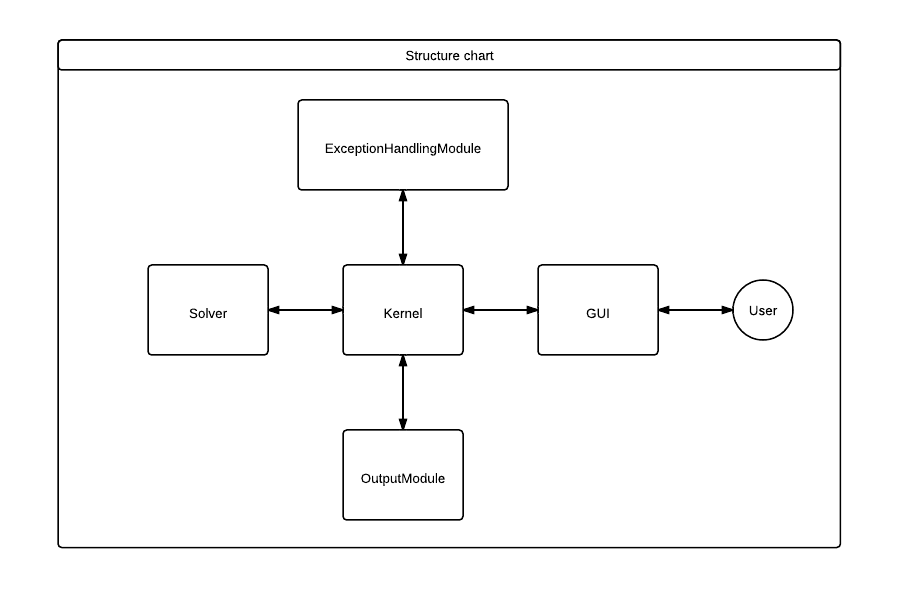
\includegraphics[width=4in,keepaspectratio=true]{figures/StructureDiagGyroSim.png}

\section{Detailentwurf: Klassen}
\label{sec:3.2}
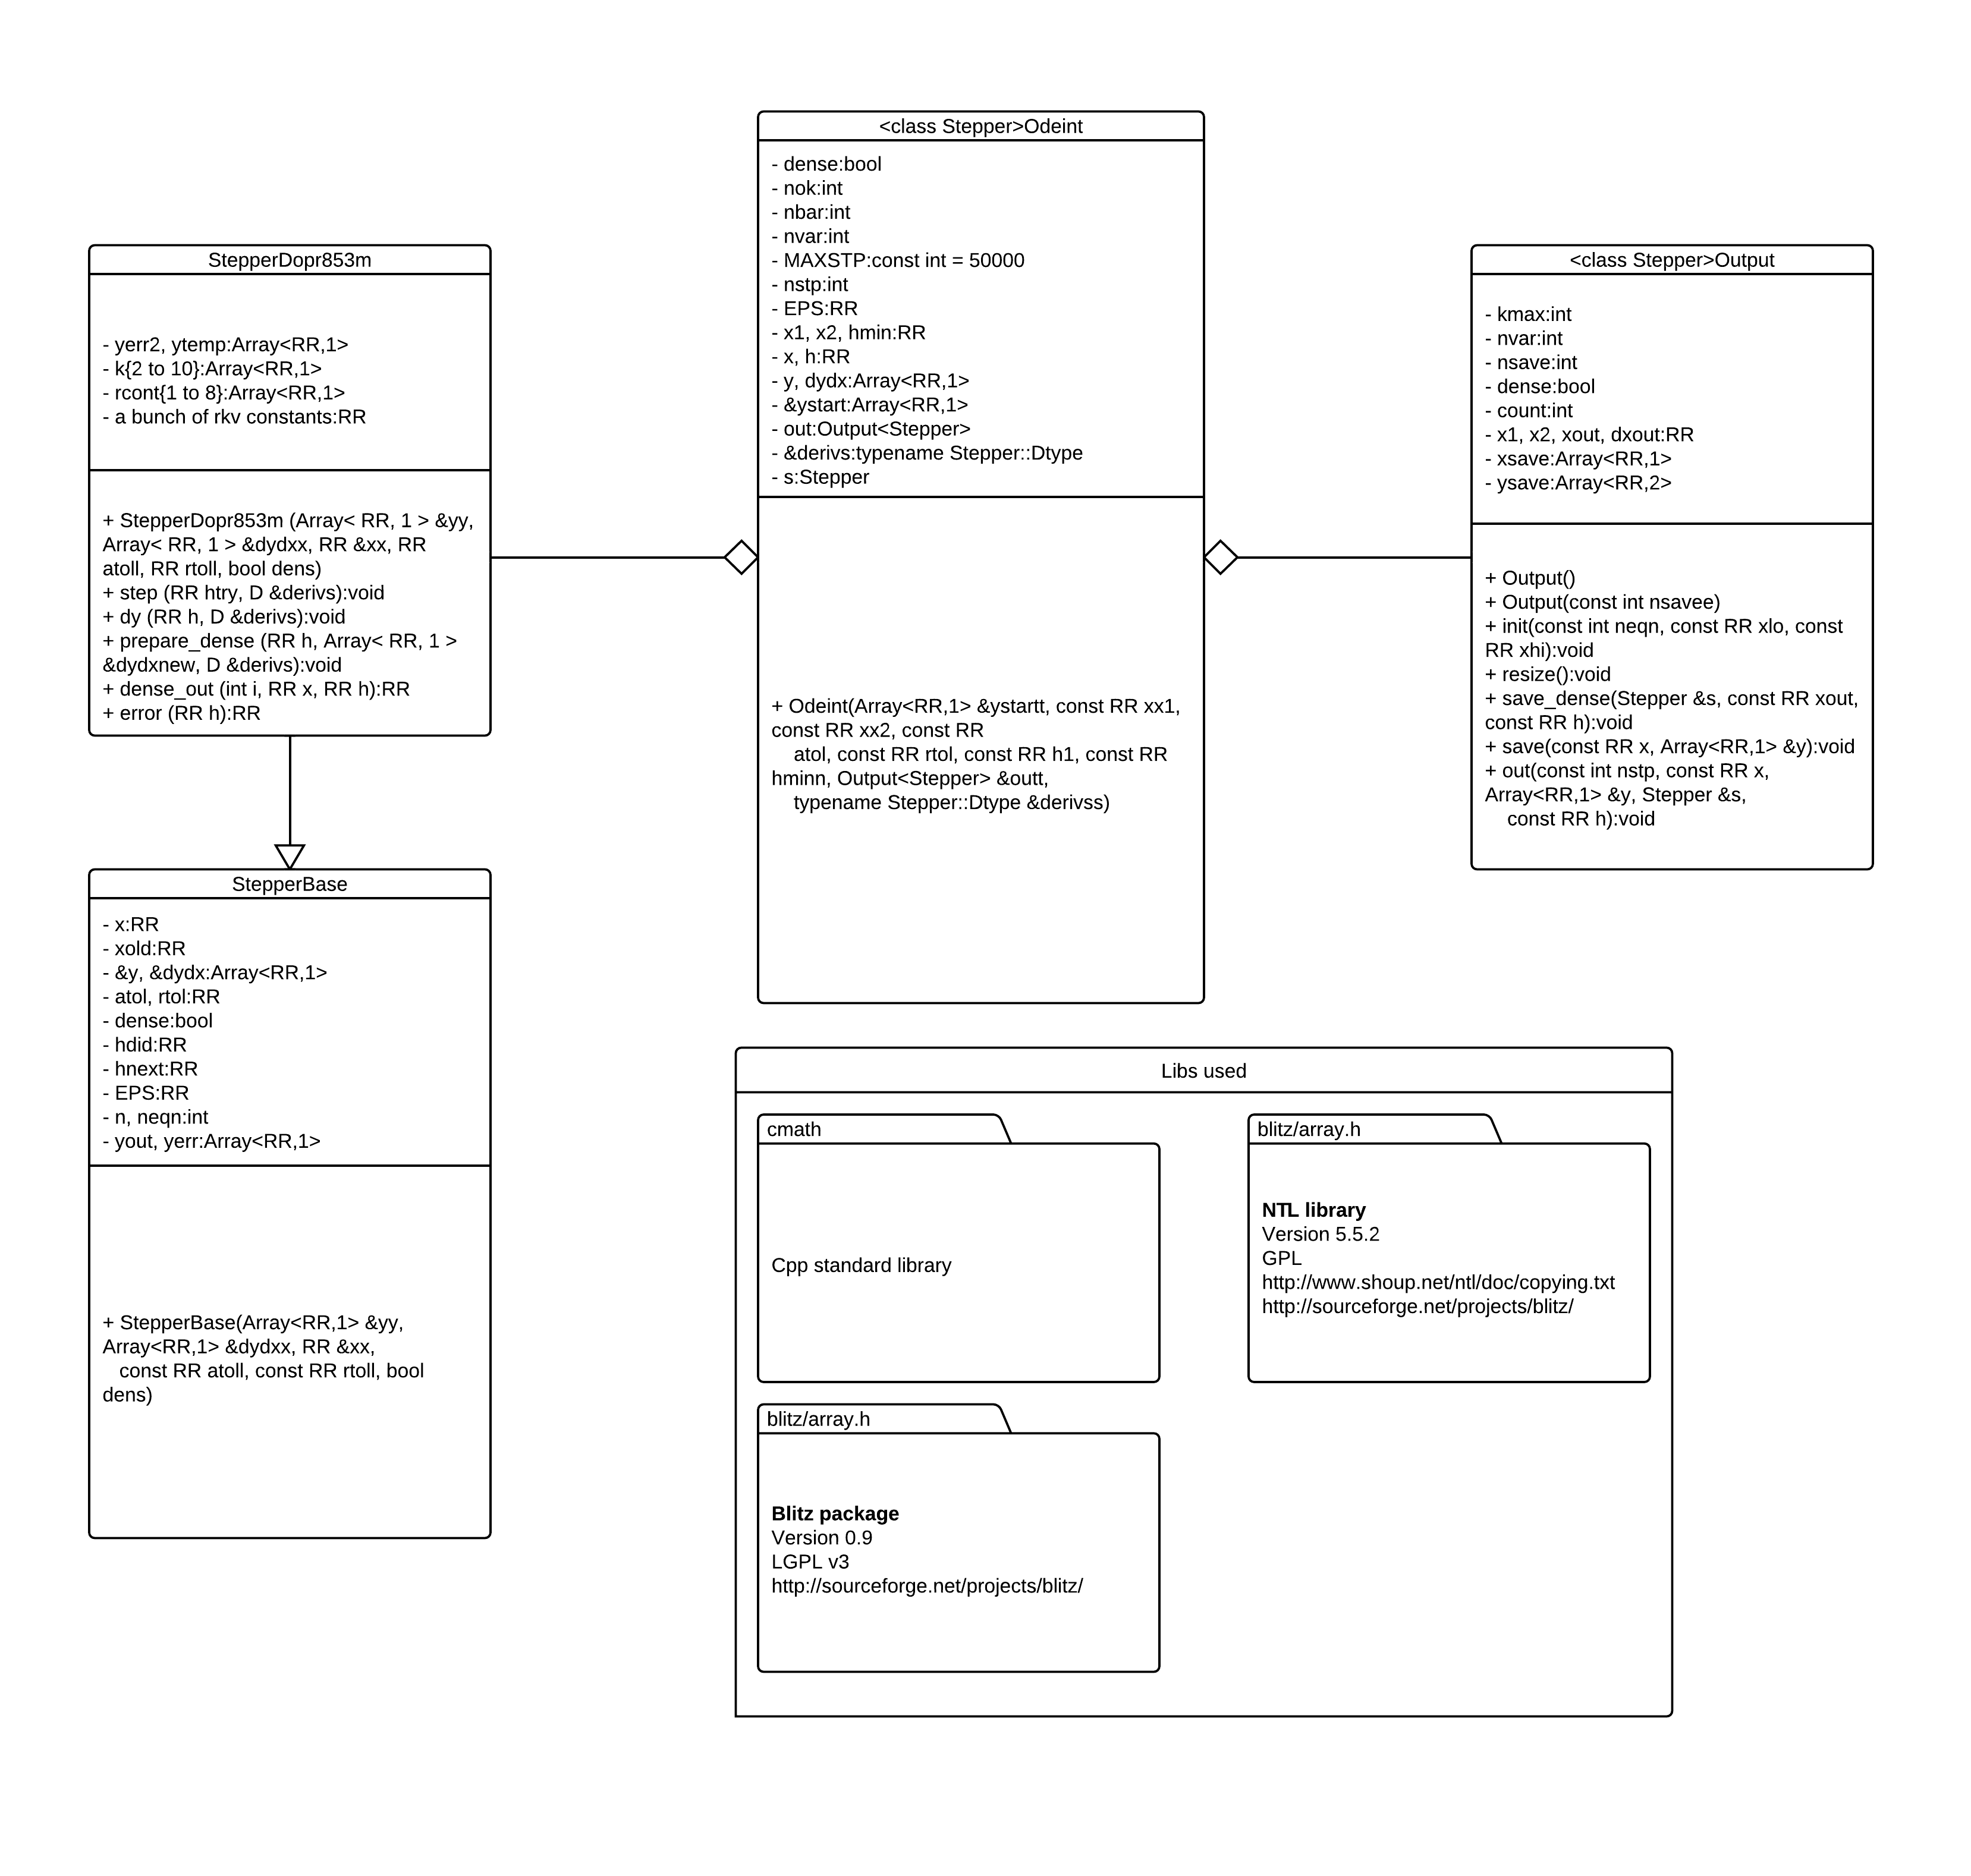
\includegraphics[width=4in,keepaspectratio=true]{figures/klassenidagramm.png}
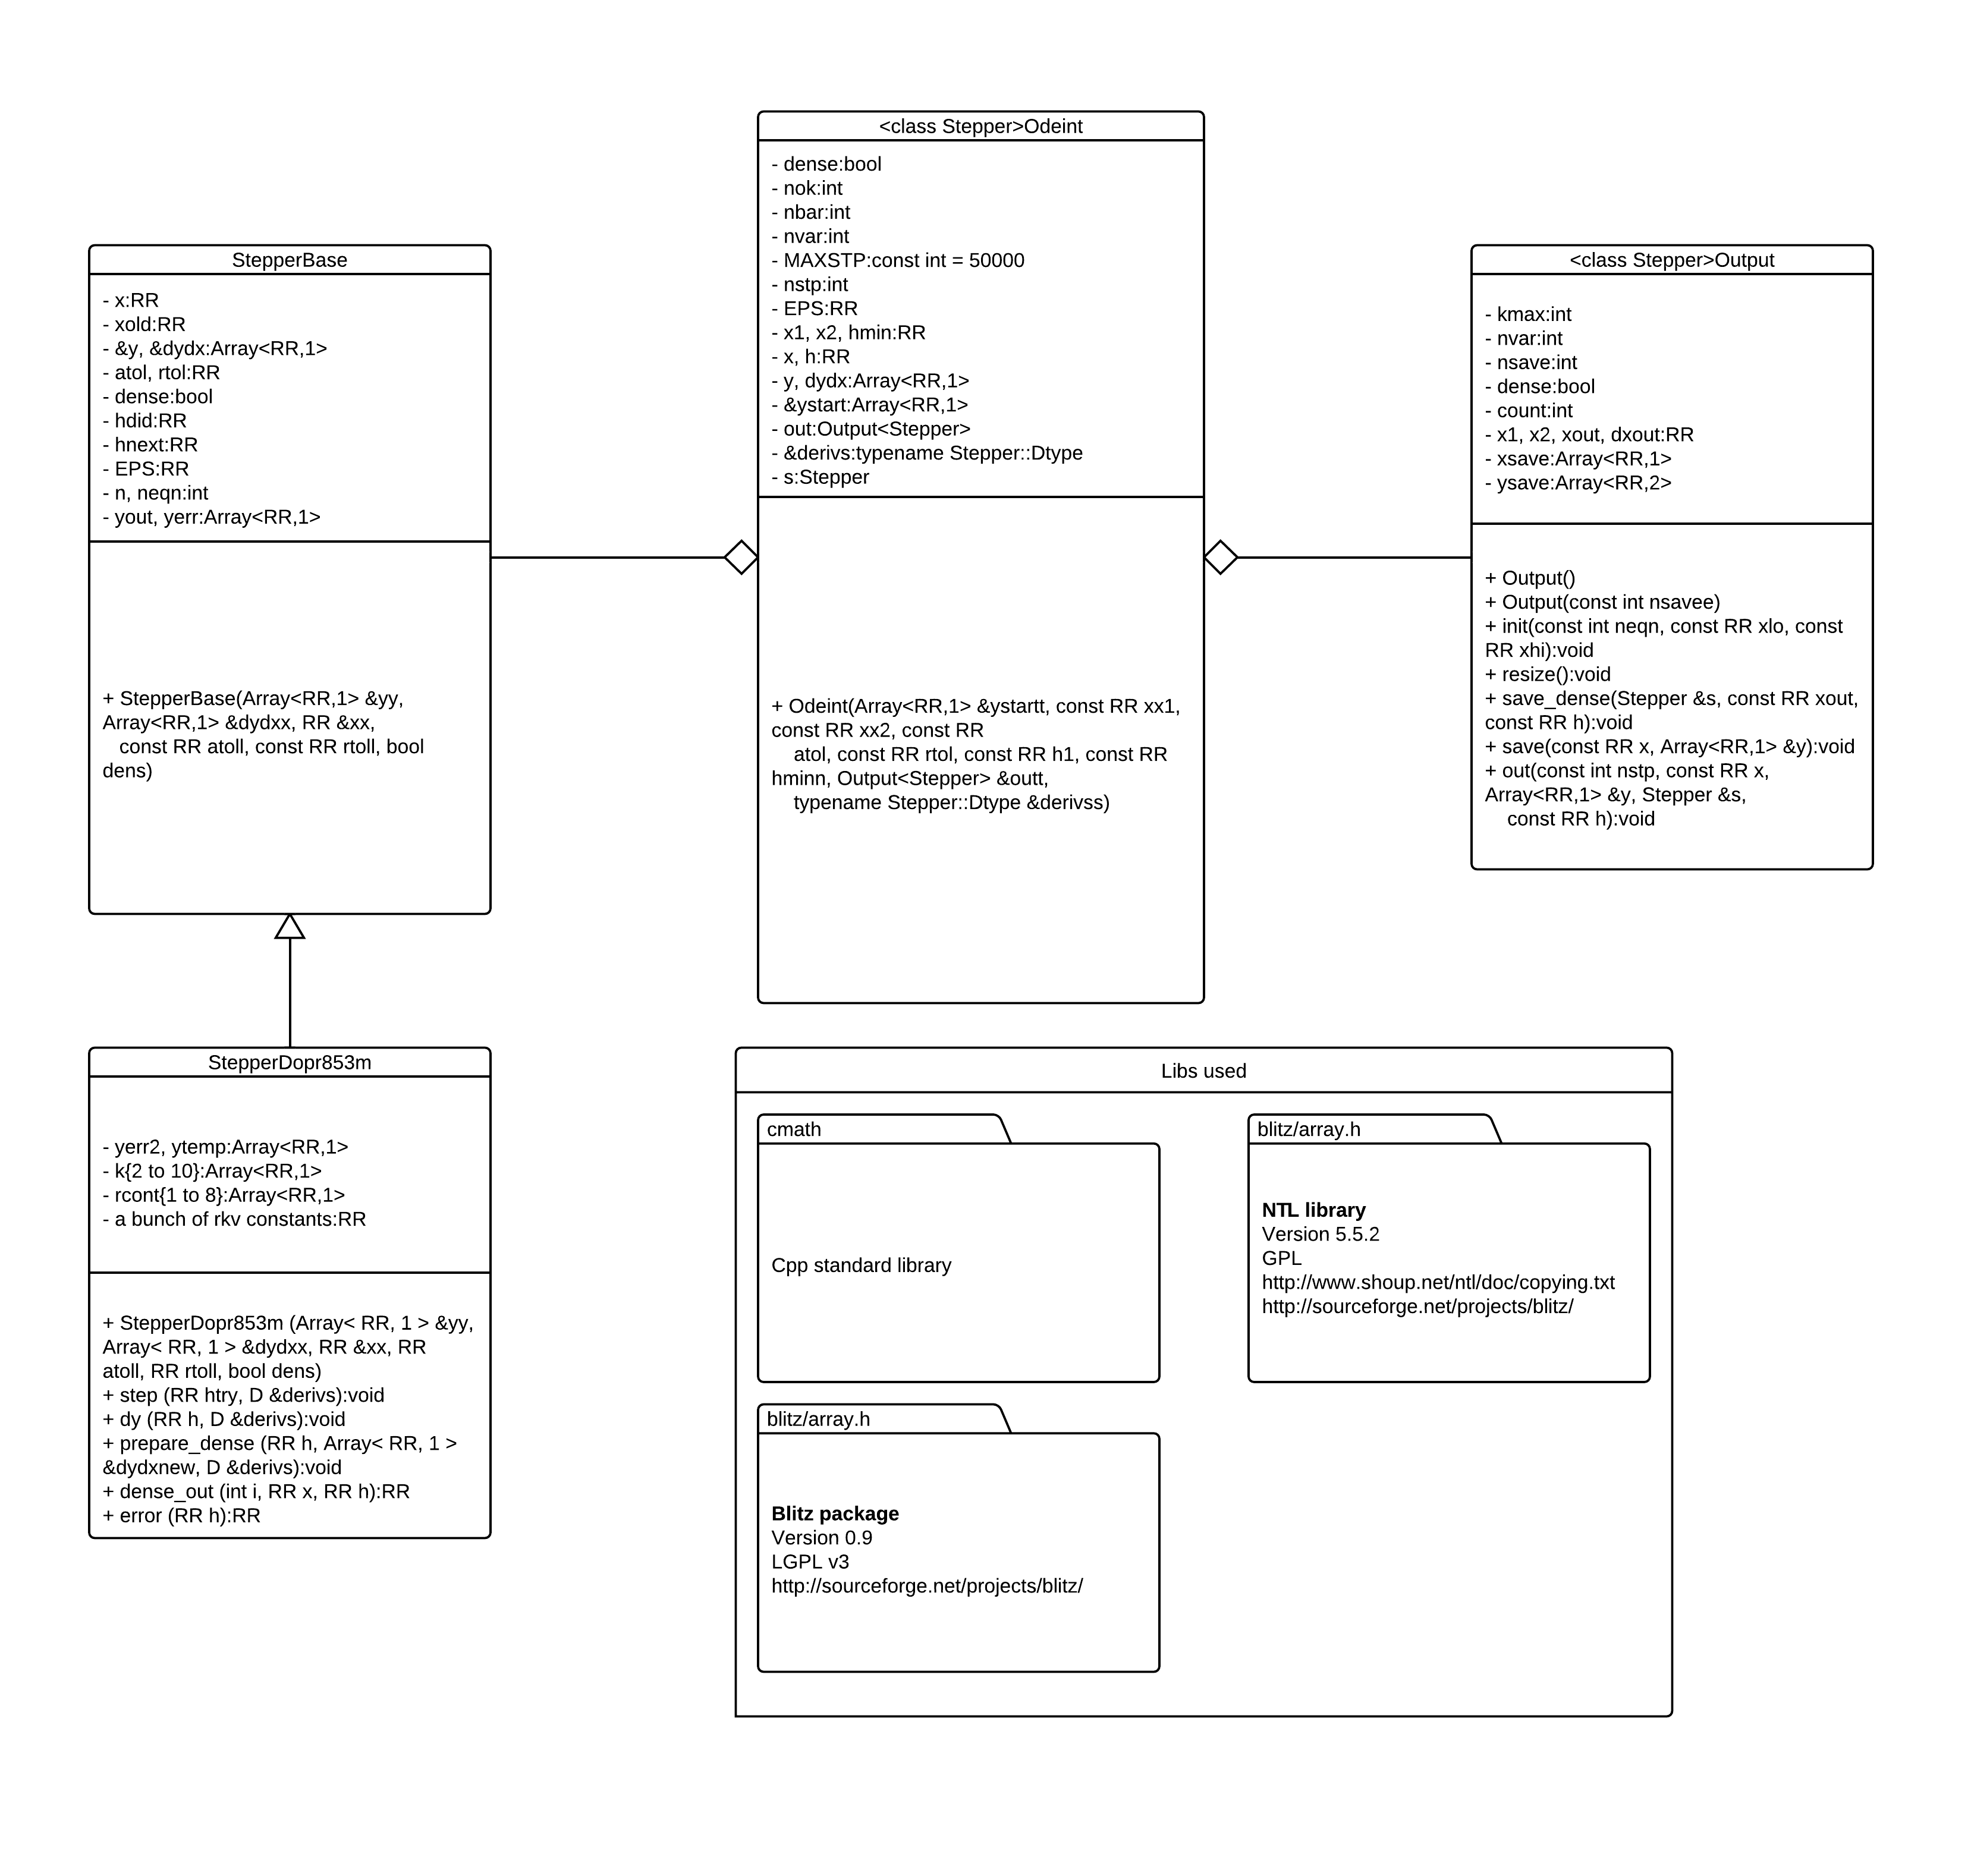
\includegraphics[width=4in,keepaspectratio=true]{figures/Odeint.png}

\subsection*{StepperDopr853 - Dormand-Prince 853 method}
Entwicklungsschritte vom Prototypen zum fertigen L\"oser

Um Referenzdaten erzeugen zu k\"onnen und fr\"uhzeitig mathematische Fehler ausschlie\ss en zu k\"onnen haben wir uns f�r die Implementierung eines Prototypen entschieden.
Nach der ersten Implementierung eines rkv56 Verfahrens in Matlab entschieden wir uns, zu Gunsten einer h\"oheren Genauigkeit und Geschwindigkeit, weiter Implementierungen in Fortran95 zu programmieren.

Der fertige Fortran Prototyp, ebenfalls ein Runge-Kutta 56 mit adaptiver Schrittweitensteuerung, ben\"otigte f�r die L\"osung des TippeTop Problems\footnote[1]{$k=0.3, h_{min}=10^{-8}, h_{max}=10^{-6}, rtol=atol=10^{-4}, y0=(0.0, 0.0, 250.0, 0.0, 0.0, 0.1, 0.0, 0.0, 0.0, 0.0), T=[0,2.75], dG <10^{-6}, 3160922$ Einzelschritte.} \medskip

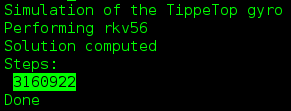
\includegraphics[width=2in,keepaspectratio=true]{figures/dopr0.png}

L\"osung des Prototypen f�r $\dot\psi$ in $rot/s$ \medskip

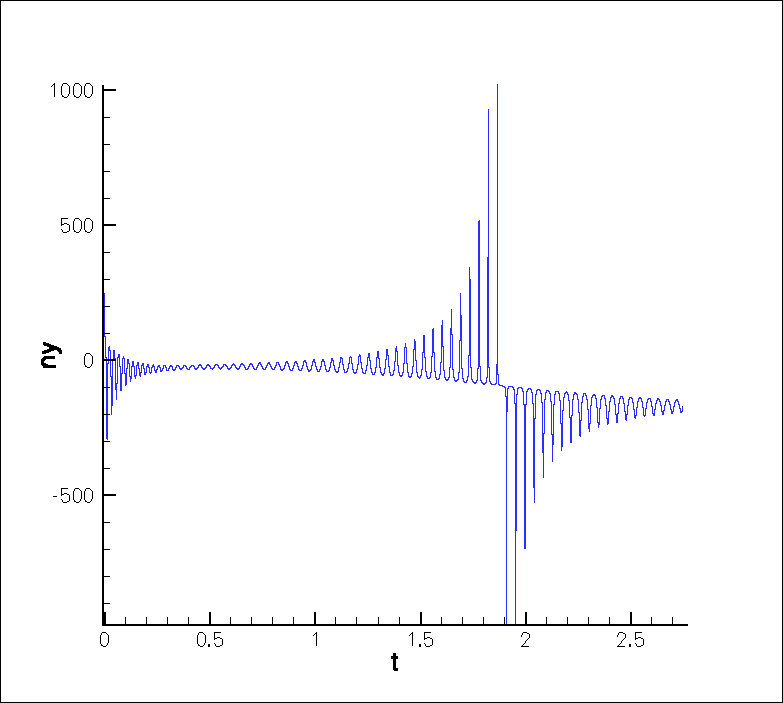
\includegraphics[width=4in,keepaspectratio=true]{figures/dopr1a.png}

Auf Grund der Erfahrung mit dem Prototypen entschieden wir uns f�r die Verwendung eines Dopr853 Verfahrens. Die erste Implementierung unter Verwendung des Datentyps double (auf ~15 Nachkommastellen genau) lieferte leider signifikant falsche Ergebnisse \medskip

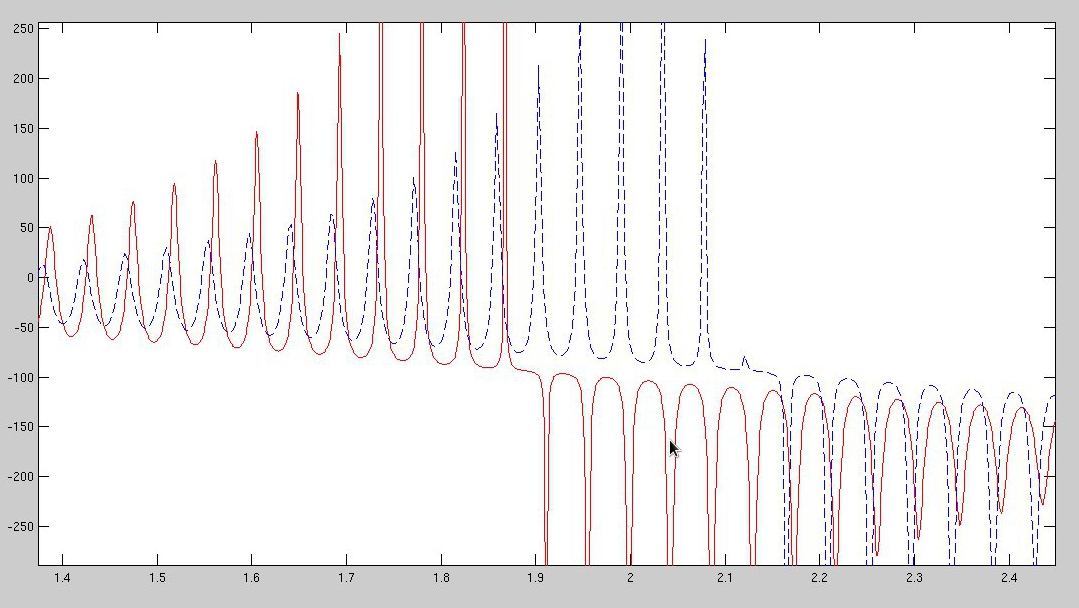
\includegraphics[width=4in,keepaspectratio=true]{figures/dopr1.png}

Die korrekte L\"osung der rkf56 Fortran95 Implementierung ist rot dargestellt, die falsche L\"osung des Dopr853$\_$double Algorithmus in blau. Es lag nahe das diese Unterschiede in der L\"osung auf Ungenauigkeiten in der Auswertung der steifen rechten Seite und den Berechnungen des Dopr853 Algorithmus zur\"uckzuf\"uhren waren. Wir entschieden uns also f�r die Verwendung eines genaueren Datentyps, und zwar NTL::RR aus der NTL library\footnote[2]{http://www.shoup.net/ntl/}

Unter verwendung des NTL::RR Datentyps kann der fertige L\"oser (Dopr853 in \textit{C++}) die L\"osung des Problems$^1$ in 852 Schritten berechnen.

L\"osung f�r $\dot\psi$(Drehgeschwindigkeit) mit Dopr853: \medskip

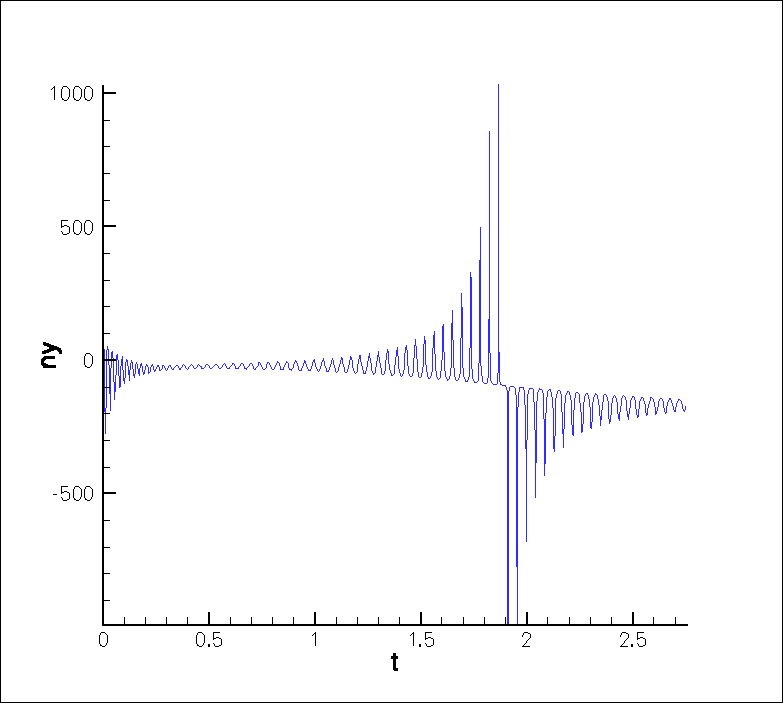
\includegraphics[width=4in,keepaspectratio=true]{figures/dopr2.png}

Der Dopr853 Algorithmus ist ein Algorithmus aus der Familie der Runge-Kutta Algorithmen der Ordnung 8.  F�r jeden Schritt werden 12 Auswertungen der rechten Seite des DGL ben\"otigt.
Der urspr\"ungliche Algorithmus nutzte eine Fehlersch\"atzung der Ordnung 6, was sich allerdings in einigen F\"allen als unzureichend herausstellte, da dieser Fehlersch\"atzer jeweils die letzte Auswertung nicht ber\"ucksichtigte. Hairer, N\"orsett und Wanner1 konstruierten Absch\"atzungen der f\"unften und dritten Ordnung, die auch den letzen Punkt ber\"ucksichtigen. Der Fehler kann also \"uber \\
$err = err_5 \frac{err_5}{\sqrt{(err_3)^2+0.01(err_5)^2}}$ \\
abgesch\"atzt werden. 

Die meiste Zeit \"uber gilt $err_5 << err_3$ und damit $err=O(h^8)$. \medskip

StepperDopr853 wurde als Mehrschrittverfahren mit fehlergesteuerter Schrittweitensteuerung implementiert, die neben dem gesch\"atzten Fehler auch noch die Erhaltungsgr\"o\ss e \\
$IR\dot\phi\sin^2\theta+I_3(R\cos\theta-a)(\dot\phi\cos\theta+\dot\psi) = const =: G$ \\
ber\"ucksichtigt. ($\Delta G$ pro Schritt $< 1E-6$ ).
Der L\"oser unterst\"utzt sowohl eine dichte Ausgabe \textit{dense output}, als auch die Ausgabe von n \"aquidistant verteilten Werten. 

\textit{Frei nach NumericalRecipes3rdEdition - Chapter 17.2.4 Dopr853 - An Eight-Order Method} \medskip

\textit{Implementierung nach Numerical Recipes Software 2007, "Routine Implementing an Eighth-order Runge-Kutta Method,"
Numerical Recipes Webnote No. 20, at http://www.nr.com/webnotes?20}
\footnote[3]{Hairer, E., N�rsett, S.P., and Wanner, G. 1993, Solving Ordinary Differential Equations I. Nonstiff 
Problems, 2nd ed. (New York: Springer). Fortran codes at 
http://www.unige.ch/~hairer/software.html }

\section{Graphical User Interface}
\label{sec:3.3}
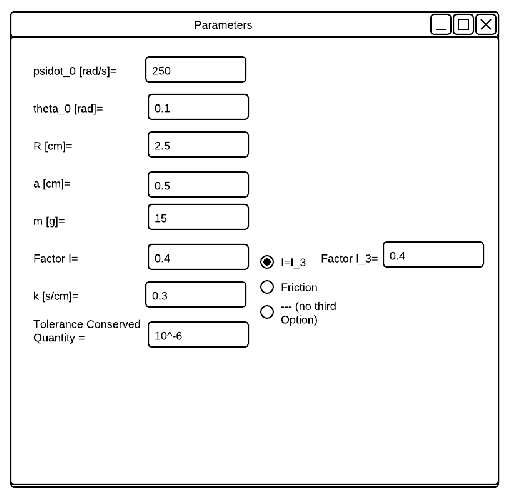
\includegraphics[width=4in,keepaspectratio=true]{figures/GUIParameterInputForm.png}
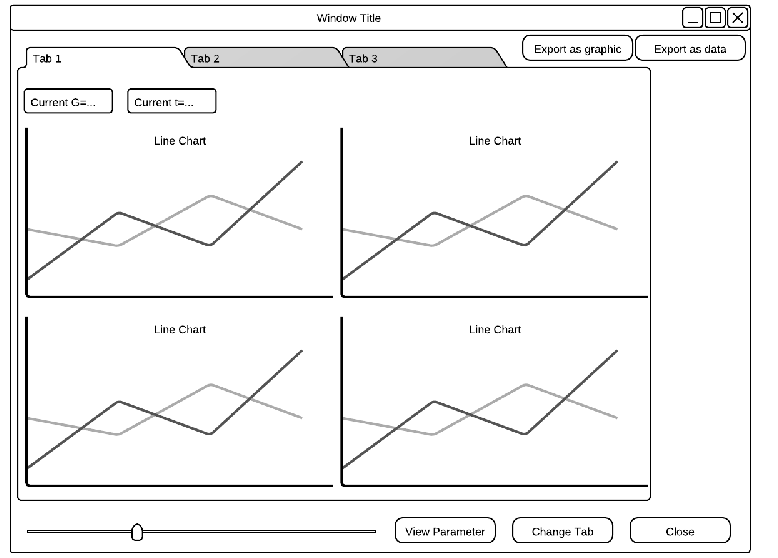
\includegraphics[width=4in,keepaspectratio=true]{figures/GUIDisplayForm.png}
\section{Use-Case-Diagramm}
\label{sec:3.4}
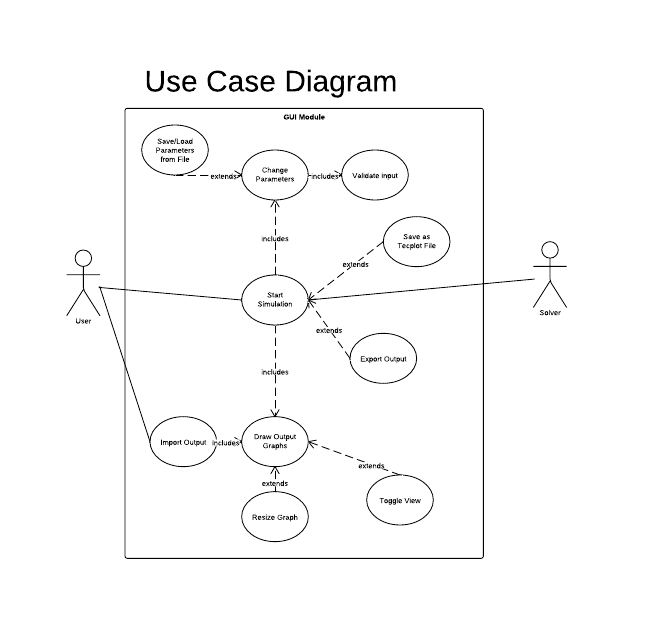
\includegraphics[width=4in,keepaspectratio=true]{figures/UseCaseTippeTop.png}


%% \chapter{Benutzerdokumentation}
\label{ch:4}

{\em - folgt -}

%% \chapter{Entwicklerdokumentation}
\label{ch:5}

%{\em wohlstrukturierte und gut lesbare Dokumentation der Software aus 
%Entwicklersicht; zahlreiche Referenzen nach \refchapter{ch:3} und in den
%Quellcode in \refchapter{ch:6}} \\
%\\
%Die Signatur der Funktion {\tt foo} finden Sie in Zeile~\ref{zn_bar} des Quellcodes~\ref{klasse1.1.hpp} in \refsec{ssec:6.1.1}.


%% \bibliographystyle{plain}
%% \bibliography{analyse_entwurf}

\appendix

\chapter{Quellcode}
\label{ch:6}

{\em einfach referenzierbare Version des Quelltexts} 

\section{Paket 1}
\label{sec:6.1}

\subsection{Klasse 1.1}
\label{ssec:6.1.1}

\begin{lstlisting}[caption=Dokumentierter Quellcode in {\tt klasse1.1.hpp},label=klasse1.1.hpp]
class foo {
  public:
    int bar(const float& f); /*@\label{zn_bar}@*/
}
\end{lstlisting}

\subsection{Klasse 1.2}

\section{Paket 2}

\section{Paket 3}



\end{document}

